%%==================================================
%% chapter01.tex for BIT Master Thesis
%% modified by yang yating
%% version: 0.1
%% last update: Dec 25th, 2016

%% modified by Meng Chao
%% version: 0.2
%% last update: May 29th, 2017
%%==================================================
\chapter{绪论}
\label{chap:intro}

\section{论文研究目的与意义}

There is a growing tendency for Real-time Monocular Simultaneous Localization and Mapping (SLAM) and 3D reconstruction. It is popular for robotics industrial, in particular to navigate unmanned aerial vehicles (UAVs) or augmented and virtual reality applications slowly making their way into the mass-market.

One of the significant benefits of monocular SLAM, simultaneously one of the biggest challenges, come with the scale-ambiguity which is that the scale of the real world cannot be observed and drift over time and become the majority error source origin. But the advantage is that this allows to switch between differently scaled environments, such as indoor and outdoor. The traditional sensors have a limited range which is that they cannot flexible and reliable measure, such as depth or stereo cameras.


\section{无人机定位技术发展现状}


\section{视觉SLAM发展现状}



\section{论文主要内容和结构安排}




\begin{figure}
  \centering
  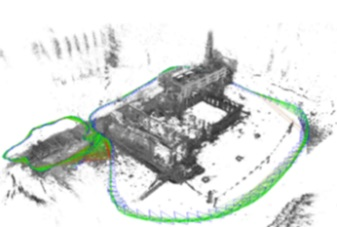
\includegraphics[height=0.5\textwidth]{figures/Fig1(1)}
  %\caption{The UAV equipped with an ASUS Xtion Pro Live RGB-D camera}
  %\label{Figure1.};
  
  \centering
  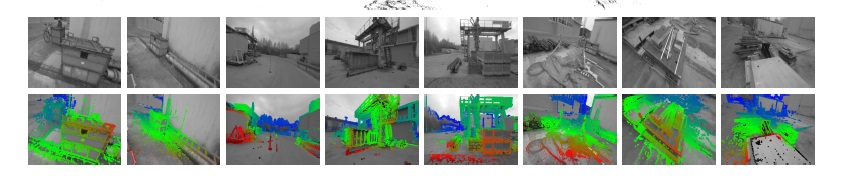
\includegraphics[width=0.75\textwidth]{figures/Fig1(2)}
  \caption{LSD-SLAM generates a consistent global map}
  %\label{referencename};
\end{figure}

The Large-Scale Direct monocular SLAM not only locally tracks the motion of the camera, but also allows to build consistent, large-scale maps of the environment (Fig.1) in \upcite{[1]} . Compared the traditional Monocular SLAM using feature-based methods, this method uses direct image alignment coupled with filtering-based estimation of semi-dense depth maps [2]. The global map is represented as a pose graph consisting of key frames as vertices with 3D similarity transforms as edges, elegantly incorporating changing scale of the environment and allowing to detect and correct accumulated drift.






\iffalse
%\section{本论文研究的目的和意义}

近年来,随着人们生活水平的不断提高,人们越来越注重周围环境对身体健康的影响。作为服装是人们时时刻刻最贴近的环境,尤其是内衣,对人体健康有很大的影响。由于合时刻刻最贴近的环境,尤其是内衣,对人体健康有很大的影响。由于合成纤维的衣着舒适性、手感性,天然纤维的发展又成为人们关注的一大热点。
%\upcite{Takahashi1996Structure,Xia2002Analysis,Jiang1989,Mao2000Motion,Feng1998}

%\section{国内外研究现状及发展趋势}
%\label{sec:***} 可标注label

%\subsection{形状记忆聚氨酯的形状记忆机理}
%\label{sec:features}

形状记忆聚合物(SMP)是继形状记忆合金后在80年代发展起来的一种新型形状记忆材料\upcite{Jiang2005Size}。形状记忆高分子材料在常温范围内具有塑料的性质,即刚性、形状稳定恢复性;同时在一定温度下(所谓记忆温度下)具有橡胶的特性,主要表现为材料的可变形性和形变恢复性。即“记忆初始态-固定变形-恢复起始态”的循环。

固定相只有物理交联结构的聚氨酯称为热塑性SMPU,而有化学交联结构称为热固性SMPU。热塑性和热固性形状记忆聚氨酯的形状记忆原理示意图如图\ref{fig:diagram}所示

\begin{figure}[!htp]
 \centering
 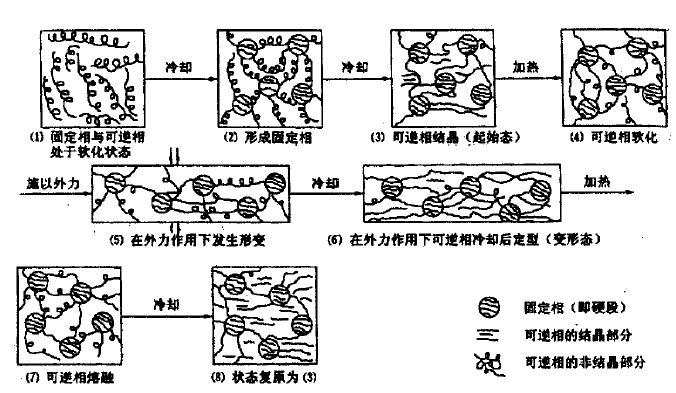
\includegraphics[width=0.75\textwidth]{figures/figure1}
 \caption{热塑性形状记忆聚氨酯的形状记忆机理示意图}\label{fig:diagram}
\end{figure}


%\subsection{形状记忆聚氨酯的研究进展}
%\label{sec:requirements}
首例SMPU是日本Mitsubishi公司开发成功的近年来,随着人们生活水平的不断提高,人们越来越注重周围环境对身体健康的影响。作为服装是人们时时刻刻最贴近的环境,尤其是内衣,对人体健康有很大的影响。由于合时刻刻最贴近的环境,尤其是内衣,对人体健康有很大的影响。由于合成纤维的衣着舒适性、手感性,天然纤维的发展又成为人们关注的一大热点。


%\subsection{水系聚氨酯及聚氨酯整理剂}

水系聚氨酯的形态对其流动性,成膜性及加工织物的性能有重要影响,一般分为三种类型\upcite{Jiang2005Size} ,如表 \ref{tab:category}所示。

\begin{table}[!hbt]
  \centering
  \caption{水系聚氨酯分类} \label{tab:category}
  
  \begin{tabular*}{0.9\textwidth}{@{\extracolsep{\fill}}cccc}
  \toprule
    类别			&水溶型		&胶体分散型		&乳液型 \\
  \midrule
    状态			&溶解$\sim$胶束	&分散		&白浊 \\
    外观			&水溶型		&胶体分散型		&乳液型 \\
    粒径$/\mu m$	&$<0.001$		&$0.001-0.1$		&$>0.1$ \\
    重均分子量	&$1000\sim 10000$	&数千$\sim 20万$ &$>5000$ \\
  \bottomrule
  \end{tabular*}
\end{table}

由于它们对纤维织物的浸透性和亲和性不同,因此在纺织品染整加工中的用途也有差别,其中以水溶型和乳液型产品较为常用。另外,水系聚氨酯又有反应性和非反应性之分。虽然它们的共同特点是分子结构中不含异氰酸酯基,但前者是用封闭剂将异氰酸酯基暂时封闭,在纺织品整理时复出。相互交联反应形成三维网状结构而固着在织物表面。
……
\fi
